% ======================================== Début Préambule Latex ========================================
% Copyright (c) 2022 Mathis Gauthey
% This source code is licensed under the MIT License found in the
% LICENSE file in the root directory of this source tree.

% ========== Classe du document ==========
\documentclass[a4paper,11pt,fleqn]{report}    % A4, police taille 11, report pour avoir les chapitres, fleqn pour avoir les équations alignées à gauche

% ========== Langue française pour le document ==========
\usepackage{latexsym}       % Police latex de base

\usepackage[french]{babel}  % Dictionnaire français (indentation, caractères spéciaux, tirets...)
\usepackage[utf8]{inputenc} % Encodage d'entrée pour les caractères accentués
\usepackage[T1]{fontenc}    % Affichage correct des caractères accentués notamment

% ========== Géométrie du document ==========
% Gestion des différentes marges du document pour coller avec le séparateur d'en-tête
\usepackage[left=2cm , right=2cm, bottom=2cm, top=2cm, headheight=2cm, headsep=0.5cm,heightrounded=true]{geometry}
% \raggedbottom % This makes the last line of each page be at exactly the same place on the sheet of paper
% \flushbottom  % All pages will not necessarily have exactly the same height, but ‘almost the same height’
\setlength{\parskip}{1em}   % Définition de l'espace entre les paragraphes
\setlength{\parindent}{4em} % Définition de la longueur du "tab" = indentation
\usepackage{fancyhdr}       % Permet en-tête et pied de page
\pagestyle{fancyplain}      % Pour avoir le même style sur les pages fancy et sur celles plains comme la toc
\renewcommand\plainheadrulewidth{.4pt}  % Le trait noir sous les logos sur les pages plain
\fancyhead[L]{
\includegraphics[scale=0.05]{logo_iresne.png}}    % Logo gauche
\fancyhead[R]{
\includegraphics[scale=0.05]{polytech.jpg}} % Logo droit
% Redéfinir le style "empty" utilisé par le documentclass "report" pour le titre, résumé et chapitres
\fancypagestyle{empty}
{
    \fancyhf{}
    \fancyhead[L]{
\includegraphics[scale=0.05]{logo_iresne.png}}    % Logo gauche
    \fancyhead[R]{
\includegraphics[scale=0.05]{polytech.jpg}} % Logo droit
}

% ========== Liens dans le document, méta-datas et références ==========
\usepackage{xpatch}     % Permet de patcher certaines fonctionnalités de base comme la toc
\usepackage{float}      % Placement des flottants
\usepackage{hyperref}   % Liens dans le documents
\usepackage{caption}    % Légendes dans les environnements "figure" et "float"
\usepackage[list=true]{subcaption} % Légendes pour les "sous-figures" et "sous-float"
                                   % et affichage des "sous-..." dans la liste des figures
%\def\thechapter{\Alph{chapter}}    % Définition des chapitres avec une lettre
\setcounter{tocdepth}{3}           % Profondeur de numérotation de la toc  (chap > sec > subsec > subsubsec)
\setcounter{secnumdepth}{3}        % Profondeur de numérotation des titres (chap > sec > subsec > subsubsec)
\usepackage{chngcntr}              % Permet de changer les numérotations d'objets
\usepackage[titles]{tocloft}       % Gestion très précise des différentes listes

\hypersetup % Attribution des méta-datas pdf pour reconnaissance automatique Zotero entre autres
{
pdftitle={Titre},
pdfsubject={Sujet},
pdfauthor={Auteur},
	pdfkeywords={keyword1} {keyword2} {keyword3}
}

% ========== Graphique, police, maths ==========
\usepackage[table,xcdraw]{xcolor}       % Package permettant d'utiliser de la couleur
% \usepackage{color}                      % Rajouter de la couleur au texte
\usepackage{bm}                         % Mettre en gras des maths avec la commande \bm
\usepackage{ragged2e}                   % Meilleure gestion de l'alignement des textes entre autres
\usepackage{tcolorbox}                  % Boite colorées pour texte, images ou équations
\usepackage{textcomp}                   % Symboles et polices
\usepackage{gensymb}                    % Symbole pour le degré entre autre
\usepackage{amsmath,amsfonts,amssymb}   % Écrire des maths
\usepackage{cancel}                     % Barrer des maths
\usepackage{mathtools}                  % Gestion des matrices et de maths complexes
\usepackage{morewrites}                 % Résoud un problème entre les listes équation et codes


\usepackage{lmodern}
\usepackage[Lenny]{fncychap}

\ChNameUpperCase
\ChNumVar{\fontsize{40}{42}\usefont{OT1}{ptm}{m}{n}\selectfont}
\ChTitleVar{\Huge \bfseries}

\usepackage{pifont}
\usepackage{enumitem}       % Gestion des énumérations

% Gestion des espaces avant et après les listes plus agréable à la vue
% \setlist[itemize]{noitemsep, topsep=5pt, before={\vspace*{-\baselineskip}}}
% Si désactivé (commenté), penser à ajouter un \smallskip, \medskip ou \bigskip après un itemize.

\definecolor{bulletcolor}{RGB}{128,128,128}


\usepackage{siunitx}                                    % Pour des unités bien écrites
\newcommand{\nomunit}[1]{%
\renewcommand{\nomentryend}{\hspace*{\fill}#1}}         % Commande pour la nomenclature (unités à droite)
\sisetup{inter-unit-product =\ensuremath{{}\cdot{}}}    % Séparation par un point des unités
\DeclareSIUnit\bar{bar}                                 % Besoin de déclarer les bar car pas pris en charge

\usepackage{contour}
\usepackage[normalem]{ulem}

\renewcommand{\ULdepth}{1.8pt}
\contourlength{0.8pt}

\newcommand{\myuline}[1]{%
	\uline{\phantom{#1}}%
	\llap{\contour{white}{#1}}%
}



% ========== Glossaire ==========
\usepackage[acronym,toc]{glossaries}    % Gestion d'un glossaire et d'une liste d'acronymes,
                                        % et ajout dans la toc de la position de ces derniers
% Pas besoin de points à la fin du document

\newglossaryentry{mot_complexe}{
    name={mot complexe},
    description={Un mot complexe nécessite généralement une explication}}

\newacronym{lfala}{LFALA}{Les Français Aiment Les Acronymes}                        % Récupère les informations du fichier glossary.tex
\makeglossaries                         % Génère le glossaire avec les informations récupérées

% ========== Nomenclature ==========
\usepackage[intoc]{nomencl}         % Gestion d'une nomenclature avec position dans la toc
\makenomenclature                   % Génère la nomenclature
\usepackage{etoolbox}               % Permet de créer des groupes de nomenclature

% Création de groupes de nomenclature : ATTENTION -> Uniquement des caractères uniques en identifiant
\renewcommand\nomgroup[1]{%
  \item[\bfseries
  \ifstrequal{#1}{A}{Groupe 1}{%
  \ifstrequal{#1}{B}{Groupe 2}{%
  \ifstrequal{#1}{C}{Groupe 3}{%
  }}}%
]} % Attention aux accolades lors de la création de groupes

\AtBeginDocument{   % Nomenclature à générer
\nomenclature[A]{$c_{air}$}{Célérité du son dans l'air à \SI{15}{\celsius} \nomunit{\SI{340.29}{\meter\per\second}}}
\nomenclature[B]{$T_N$}{Période propre de l'élément considéré}
\nomenclature[B]{\(E\)}{{Module d'Young}}
\nomenclature[C]{$\dot{\epsilon}$}{Vitesse de déformation \nomunit{\si{\per\second}}}
}

% ========== Gestion des figures ==========
\usepackage{graphicx}               % Plus d'arguments pour la fonction \includegraphics
\graphicspath{{Images/}}            % Path des images

%\counterwithin{figure}{section}     % Numérotation des figures à partir des sections
\setcounter{lofdepth}{2}            % Afficher jusqu'aux sous-figures dans la liste des figures
\cftsetindents{figure}{0em}{3.5em}  % Réglage de l'espace entre le numéro et le nom de la figure dans la liste
\setlength\cftbeforefigskip{5pt}    % Réglage de l'espacement entre les figures dans la liste
\AtBeginDocument{\renewcommand{\listfigurename}{Liste des figures}} % Renommer la liste des figures
% Ajout de la position de la liste des figures dans la toc
\xpretocmd{\listoffigures}{\addcontentsline{toc}{chapter}{\listfigurename}}{}{}

% ========== Gestion des tableaux ==========
\usepackage{array,multirow,makecell}                        % Packages utiles pour les tableaux
\setcellgapes{1pt}                                          % Paramètres sympa d'après Xm1Math
\makegapedcells                                             % Paramètres sympa d'après Xm1Math
\newcolumntype{R}[1]{>{\raggedleft\arraybackslash }b{#1}}   % Paramètres sympa d'après Xm1Math
\newcolumntype{L}[1]{>{\raggedright\arraybackslash }b{#1}}  % Paramètres sympa d'après Xm1Math
\newcolumntype{C}[1]{>{\centering\arraybackslash }b{#1}}    % Paramètres sympa d'après Xm1Math

%\counterwithin{table}{section}      % Numérotation des tableaux à partir des sections
\setcounter{lotdepth}{2}            % Afficher jusqu'aux sous-tableaux dans la liste des tableaux
\cftsetindents{table}{0em}{3.5em}   % Réglage de l'espace entre le numéro et le nom du tableau dans la liste
\setlength\cftbeforetabskip{5pt}    % Réglage de l'espacement entre les figures dans la liste
% Ajout de la position de la liste des tableaux dans la toc
\xpretocmd{\listoftables}{\addcontentsline{toc}{chapter}{\listtablename}}{}{}

% ========== Gestion des équations ==========
\newcommand{\listequationsname}{Liste des équations}    % Renommer la liste des équations
\newlistof{myequations}{equ}{\listequationsname}
\newcommand{\myequations}[1]{%
   \addcontentsline{equ}{myequations}{\protect\numberline{\theequation}#1}
}
\counterwithin{equation}{chapter}           % Numérotation des équations à partir des sections
\cftsetindents{myequations}{0em}{3.5em}     % Réglage de l'espace entre le numéro et le nom de l'équation dans la liste

% Création de la commande \noteworhty pour les équations importantes qui méritent d'être listées
\newcommand{\noteworthy}[2]{
\begin{align} \label{#2} \ensuremath{\boxed{#1}} \end{align}
\myequations{#2}
\begingroup
\centering \small \textit{#2}

\endgroup}

\makeatletter   % Espacement des équations plus important entre les chapitres
\xpretocmd{\@chapter}{\addtocontents{equ}{\protect\addvspace{10\p@}}}{}{}{}%
\makeatother





% ========== Index ==========
\usepackage{imakeidx}   % Package pour créer l'index
\makeindex              % Génération de l'index
% Ajout de la position de l'index dans la toc
\xpretocmd{\printindex}{\addcontentsline{toc}{chapter}{\indexname}}{}{}

% ========== Bibliographie ==========
% Importer un fichier biblatex, sans dépassement des marges, trié par ordre d'apparition
\usepackage[
backend=biber,
style=numeric,
sorting=none
]{biblatex}
\usepackage{csquotes}           % Gestion des caractères " " lors des citations
\addbibresource{biblio.bib}    % Importer le fichier de bibliographie
%\nocite{*}                      % Importer les éléments non cités quand même dans la bibliographie

% ========== Gestion des annexes ==========
\usepackage[toc,page,title,titletoc,header]{appendix}   % Packages indexes importants
\usepackage{pdfpages}                                   % Intégration de pdf dans le document
\renewcommand{\appendixtocname}{Table des annexes}      % Nom de la table des annexes dans la toc
\renewcommand{\appendixpagename}{Annexes}               % Nom du titre de la page des annexes
\usepackage{titletoc}	% Permet de générer une petite table des annexes

% ========== Utilitaires ==========
\usepackage[all,defaultlines=3]{nowidow}    % Macro pour la gestion des lignes seules en bout de page
\usepackage{blindtext}                      % Génération de texte aléatoire pour les exemples
% A utiliser avec https://ctan.mirror.garr.it/mirrors/ctan/macros/latex/contrib/mwe/mwe.pdf pour les images

% Paquets et commande perso clement plumecocq
\usepackage{bm}
\newcommand{\M}{\mathbb}					
\newcommand{\Mb}{\mathbf}									
\newcommand{\Mc}{\mathcal}
\newcommand{\grad}[1]{\nabla #1}
\renewcommand{\div}[1]{\nabla \cdot \left(#1\right)}
\newcommand{\Lapl}[1]{\Delta #1}
\newcommand{\boundary}[1]{\partial \domain{#1}}
\newcommand{\doubleoverline}[1]{\bar{\bar{#1}}} 			% notation matrice

\newcommand{\co}[1]{\text{cos}\left(#1\right)}
\newcommand{\sinus}[1]{\text{sin}\left(#1\right)}




% ======================================== Fin Préambule Latex ========================================

% ======================================== Début TUTOs ========================================

% ========== Intégrer une image ==========
%\begin{figure}[htbp]
%\centering
%\includegraphics[width=\textwidth]{example-image-a.png}
%\caption{Image A}
%\label{fig:example-image-a} % Bon réflexe de garder le même nom de fichier et de label
%\end{figure}

% ========== Insérer de multiples images ==========
% \begin{figure}[H]
%     \begin{subfigure}[t]{0.475\textwidth}
%         \includegraphics[width=1\textwidth]{example-image-b}
%         \caption{Image B}
%         \label{subfig:example-image-b}
%     \end{subfigure}%
%     ATTENTION, le % est très important ici pour éviter les problèmes de vide
%     \hfill    % Remplissage entre les images
%     \begin{subfigure}[t]{0.475\textwidth}
%         \includegraphics[width=1\textwidth]{example_image_c}
%         \caption{Image C}
%         \label{subfig:example-image-c}
%     \end{subfigure}
%     \caption{Exemple d'utilisation des sous-figures}
%     \label{fig:test_subfigure}
% \end{figure}

% ========== Placement des images ==========
% h Place the float here, i.e., approximately at the same point it occurs in the source text (however, not exactly at the spot)
% t Position at the top of the page.
% b Position at the bottom of the page.
% p Put on a special page for floats only.
% ! Override internal parameters LATEX uses for determining "good" float positions.
% H Places the float at precisely the location in the LATEX code. Requires the float package (\usepackage{float}). This is somewhat equivalent to h!, though some errors may arise if you have too many consecutive floats with [H].

% ========== Intégrer un tableau ==========
% https://www.tablesgenerator.com/

% ========== Intégrer une équation ==========
% https://editor.codecogs.com/
% \noteworthy{equation}{légende} pour l'avoir dans la liste des équations

% ========== Intégrer du code ==========
% \begin{listing}[htbp]
% \begin{minted}{c}
% #include <stdio.h>
% int main() {
%   printf("Hello, World!"); /*printf() outputs the quoted string*/
%   return 0;
% }
% \end{minted}
% \caption{Hello World in C}
% \label{listing:2}
% \end{listing}

% \mint{python}|print("hello")| % Équivalent de \minted mais plus court

% \mintinline{python}|print("hello")|   % Quand t'as qu'une ligne de code

% Remarque : Le séparateur aurait pu être { } ou d'autres ponctuations

% \inputminted[firstline=2, lastline=12]{octave}{BitXorMatrix.m}

% ========== Début de doc classique ==========
% \title{Titre}
% \author{Auteur}
% \date{\today}
% \maketitle
% \begin{abstract}
%     Blablabla
% \end{abstract}

% ======================================== Fin TUTOs ========================================
%---AUTRES PAQUETS---

%----------

\begin{document}

% ======================================== Début Page de Garde ========================================

\hypersetup{pageanchor=false}
\begin{titlepage}
    \begin{center}
        \vspace*{1cm}

        \Huge
        \textbf{Validation et amélioration d'un code CFD couplant hydrodynamique et transfert de masse}

        \vspace{0.5cm}
        \LARGE
        Commisariat à l'énergie atomique et aux énergies alternatives Cadarache 13115 Saint-Paul-lèz-Durance\\
        Laboratoire de Modélisation des Accidents Graves, LMAG\\
        27/02/2023 - 11/08/2023
        \vspace{1.5cm}

        \textbf{Clément Plumecocq}

        \vfill

        
\includegraphics[scale=0.15]{logo_iresne.png}
\includegraphics[scale=0.20]{polytech.jpg}

        \vfill

        \Large
        \noindent\fbox{\begin{minipage}[c][0.3\textwidth]{\textwidth-7pt}%
        \begin{center}
        POLYTECH Marseille - Mécanique Energétique
        \par\end{center}
        \begin{center}
        Maître de stage : Romain Le Tellier, Ingénieur-Chercheur LMAG \\
        Encadrant : Mirantsoa-Aimé Rasolofomanana, Doctorant LMAG \\
        Tuteur école : 
        \par\end{center}
        \end{minipage}}
    \end{center}
\end{titlepage}

% ======================================== Fin Page de Garde ========================================

% ======================================== Début Page Résumé ========================================

% French

\thispagestyle{empty}
\begin{center}
    \Large


    \vspace{0.9cm}
    \textbf{Résumé}
\end{center}

\blindtext

\begin{center}
	\Large
	\vspace{0.9cm}
	\textbf{Abstract}
\end{center}

\blindtext

% ======================================== Fin Page Résumé ========================================

% ======================================== Début TOC & Co ========================================

\newpage
\hypersetup{pageanchor=true}
\setcounter{page}{1}
\tableofcontents



\newpage
\printnomenclature

% ======================================== Fin TOC & Co ========================================

% ======================================== Début Document ========================================

\newpage
\section*{Contexte et remerciements}
\chapter{Introduction}
\chapter{Présentation des accidents graves dans les réacteurs à eau pressurisée}
\section{Fonctionnement d'un réacteur à eau pressurisée}

En France 56 réacteurs nucléaire dispersé sur 18 sites de type réacteur à eau pressurisée (REP) sont actuellement en service. Ces réacteurs représentent 70\% de la production électrique dans l'hexagone en 2019 d'après RTE et en 2018 la France a été le deuxième plus gros producteur d'énergie nucléaire après les États-Unis. Les puissances fournis par ces réacteurs varient entre 900 MWe et 1450 MWe. Les réacteurs français actuellement en fonctionnement sont dit de deuxième génération. Un réacteur de troisième génération d'une puissance de 1650 MWe (EPR - European pressurized reactor) est actuellement en construction sur le site de Flamanville, ce type de réacteur prend en compte le retour d'expérience des réacteurs actuels. La construction de 6 nouveaux EPR à été annoncé et 8 autres pourraient voir le jour. \\


Les REP sont des réacteurs de la famille des réacteurs à eau légère, de l'eau est utilisée comme fluide caloporteur et modérateur, de plus cette eau est pressurisé à 157 bar pour éviter un changement d'état liquide-gaz dans le circuit primaire et ainsi obtenir un meilleurs coefficient d'échange thermique, ainsi à l'entrée du condenseur la température du circuit primaire est de 350\textdegree C.
\begin{figure}[h!]
	\centering
	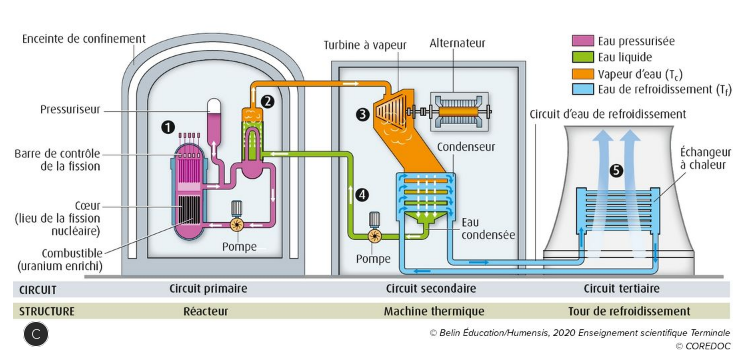
\includegraphics[width=0.8\linewidth]{figure/sch_centrale1}
	\caption[Schéma de principe d'une centrale nucléaire de type REP]{Schéma de principe d'une centrale nucléaire de type REP, (d'après manuelnumeriquemax.belin.education)}
	\label{fig:schcentrale1}
\end{figure}

\section{Sûreté des REP}
Les questions de sûreté sont intrinsèquement liées à l'exploitation d'une centrale nucléaire tant les conséquence d'un potentiel accident peuvent être importante. Ainsi dès le début des années 1970 le concept de défense en profondeur a été mis en place, ce concept se materialise par la mise en place de lignes de défense successive indépendante. Pour les REP on compte 3 barrières de confinement de la radioactivité :
 \\
\begin{minipage}[c]{0.3\linewidth}
	\begin{enumerate}
		\item La gaine combustible
		\item La cuve
		\item Le bâtiment réacteur
	\end{enumerate}
\end{minipage} \hfill
\begin{minipage}[c]{0.65\linewidth}
	\centering
	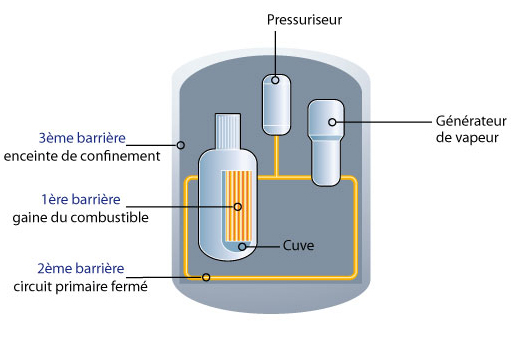
\includegraphics[width=0.7\linewidth]{figure/irsn_barriere-confinement.png}
	\captionof{figure}{Schéma des barrières de confinement (d'après irsn.fr)}
\end{minipage}
\vspace{0.5cm}


De plus les variation par rapport au régime nominal sont classés selon l'échelle INES (International Nuclear Scale Event), cette échelle permet de classifier les accident et leurs gravité, elle comporte huit échelons allant d'un simple écart (plusieurs centaines de cas par an en France) à l'accident majeur. Les accidents correspondent aux paliers 4 à 7 et se différencient de l'incident du fait de la perte d'intégrité de la première barrière résultante de la fusion du c\oe ur, le produit de cette fusion est alors appelé corium.
\begin{figure}[h!]
	\centering
	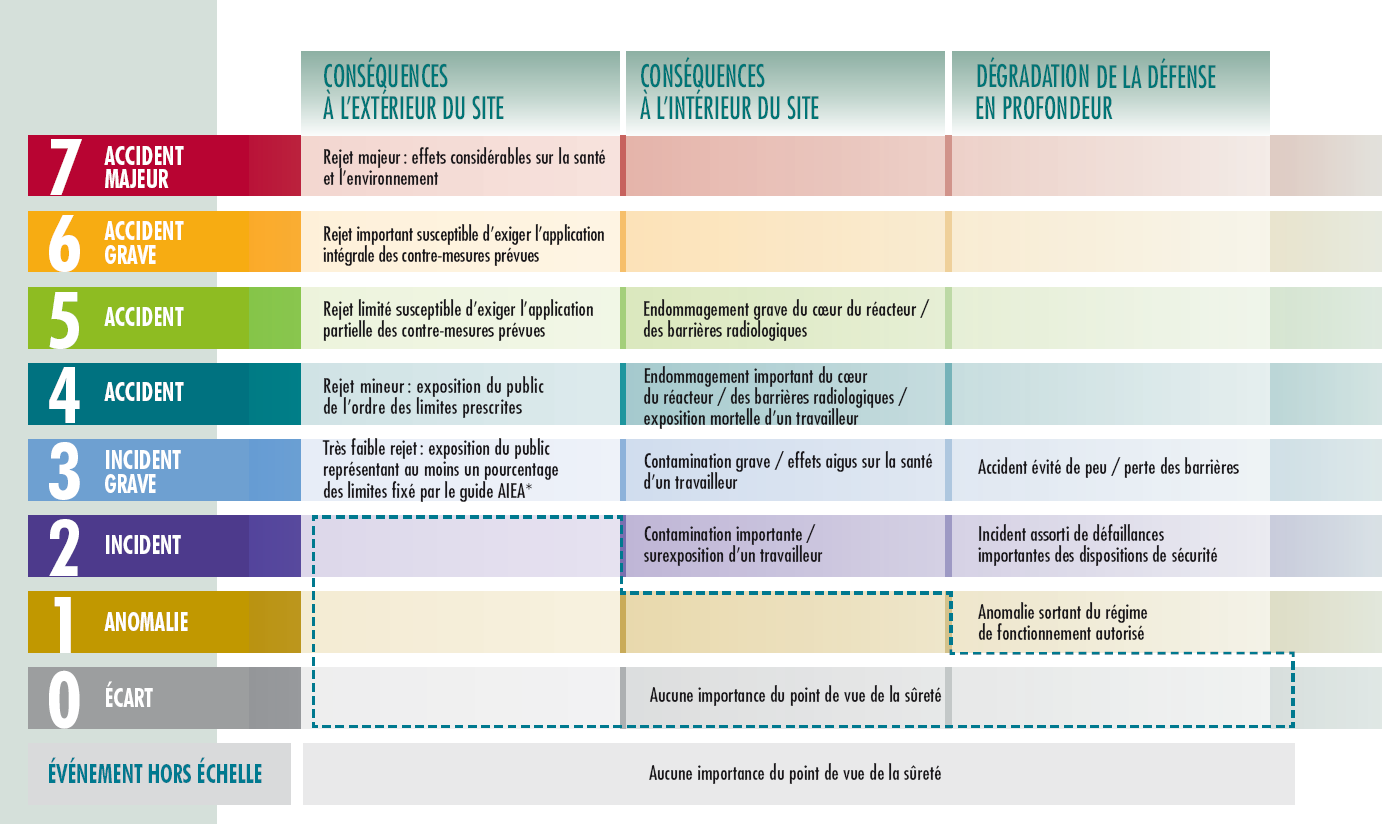
\includegraphics[width=0.7\linewidth]{figure/echelle-ines-article}
	\caption[Echelle de classification des écarts aux régimes nominal INES]{Echelle de classification des écarts aux régimes nominal INES (d'après ASN)}
	\label{fig:echelle-ines-article}
\end{figure}\\
Les accidents possible dans les REP sont séparés en deux grandes catégories, les accidents de réactivité et les Accidents de Perte de Réfrigérant Primaire (APRP). Les accidents de réactivité sont du à une accélération brutale de la réaction en chaîne entraînant une augmentation de puissance thermique produite. Les Accidents de Perte de Réfrigérant Primaire (APRP) résultent quant à eux d'une fuite dans le circuit primaire ou un arrêt de la circulation du fluide caloporteur. Dans la suite nous traiterons uniquement de cette seconde famille d'accident.
D'après \cite{kolev_multiphase_2015} voici le scénario de fonte du c\oe ur :
\begin{itemize}
	\item[] \underline{Entre 800 et 900 \textdegree C :} L'augmentation de la pression à l'intérieur de la gaine en zirconium provoque un gonflement puis une rupture de cette dernière.
	\item[] \underline{Entre 900 et 1300 \textdegree C :} Début de la réaction fortement exothermique d'oxydation de la gaine. A cet instant une forte proportion de la puissance thermique dégagée provient de cette réaction. La molécule d'eau est dissociée, l'oxygène est absorbé par la surface métallique et l'hydrogène est libéré. L'absorption de l'hydrogène dans les fissures du métal le fragilise davantage et accélère le processus de défaillance de la gaine. De plus l'apparition de fissure augmente la surface de réaction provoquant une accélération de la réaction.
	\item[] \underline{Entre 1300 et 1400 \textdegree C :} Apparition d'alliages constitués des matériaux composant la gaine (principalement Zr) et de l'acier présent dans la cuve.
	\item[] \underline{Entre 1400 et 1500 \textdegree C :} Fusion et rupture des structures métallique du c\oe ur. Libération des composant en phase gazeuse du combustible.
	\item[] \underline{Entre 1500 et 1850 \textdegree C :} Point de fusion du zirconium, dissolution du dioxyde d'uranium UO$_2$ par le zirconium en fusion, apparition de l'alliage (U,O,Zr)
	\item[] \underline{Entre 2000 et 2650 \textdegree C :} Fusion du ZrO$_2$, dissolution de l'UO$_2$ dans le ZrO$_2$ fondu et formation de la solution liquide UO$_2$-ZrO$_2$.
\end{itemize}
Une fois le c\oe ur fondu celui-ci se relocalise dans le fond de la cuve réacteur et il devient nécessaire d'adopter une stratégie pour refroidir ce bain.

\section{Traitement des accidents graves}
Une fois le c\oe ur fondu et relocalisé en fond de cuve, deux stratégies s'opposent quant à la rétention du corium : la rétention en cuve (IVR : In-Vessel Retention) ou hors cuve (EVR : Ex-Vessel Retention), la stratégie IVR présente l'avantage de garder intacte la seconde barrière de confinement contrairement à l'EVR, cependant sa mise en \oe uvre sur des réacteur de forte puissance n'est actuellement pas validée.



\chapter{Modélisation par une méthode champ de phase}
\section{Méthode d'interface diffuse}

Les méthodes de suivi d'interfaces peuvent se découper en deux principaux paradigme concernant le traitement de l'interface, cette dernière peut être raide ou diffuse. Dans le second cas l'interface est modélisé comme une zone de transition d'épaisseur connue entre les deux phases ou les deux fluides cohabitent de manière à ce que les variables observé varient de manière continu, facilitant ainsi le traitement numérique de l'interface.
\begin{figure}[h!]
	\centering
	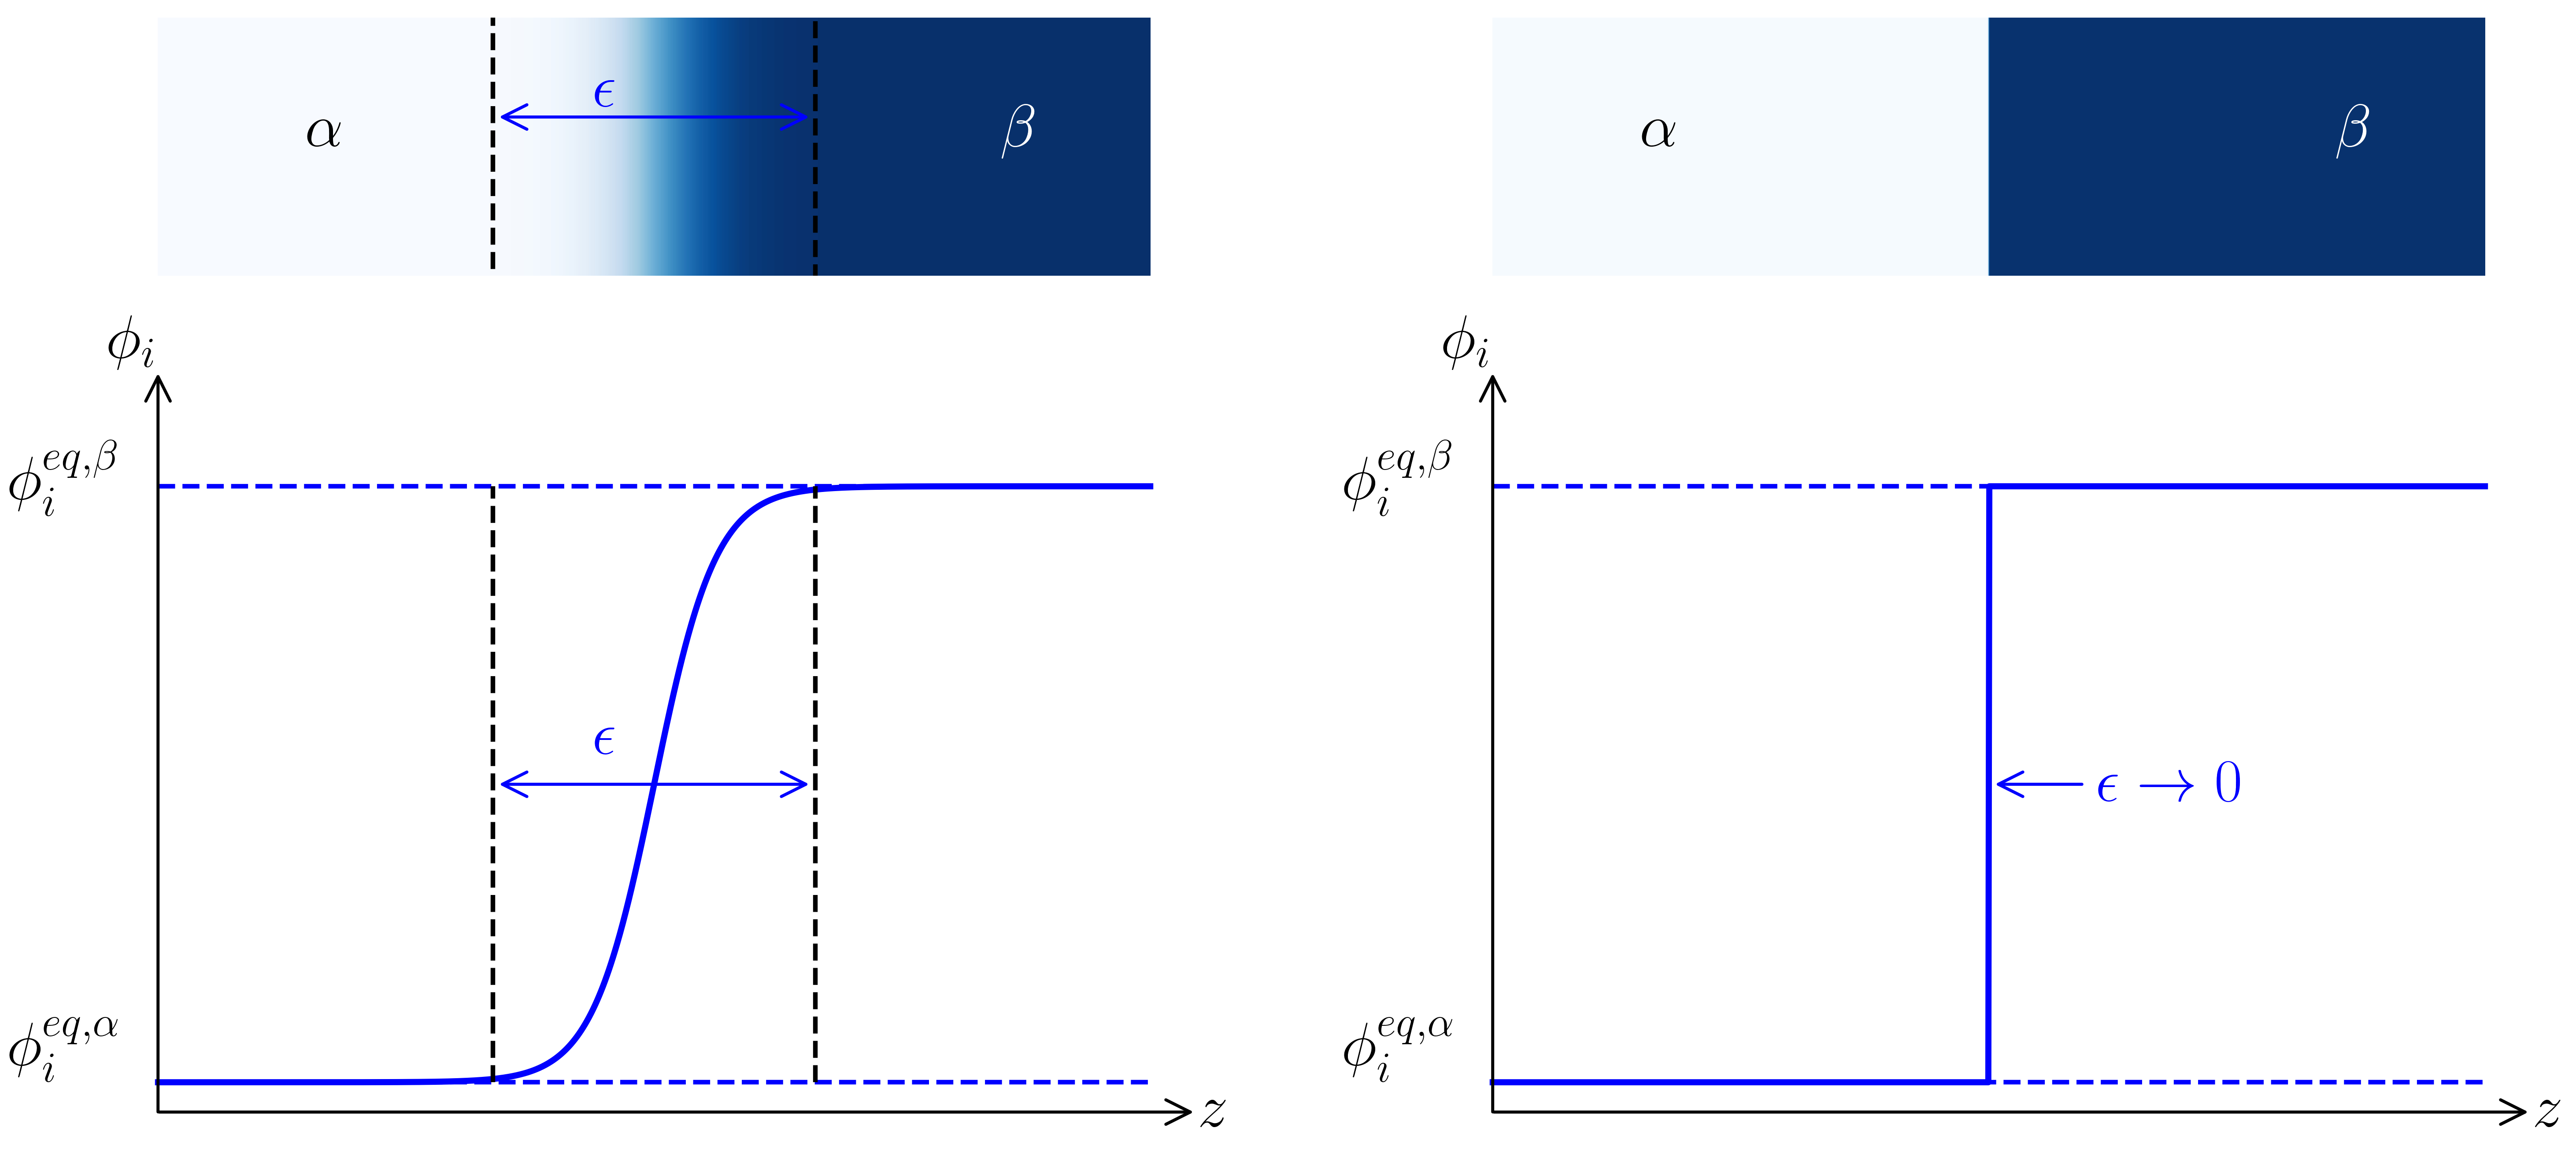
\includegraphics[width=0.3\linewidth]{figure/diffuse_interface}
	\caption[Schéma d'une interface raide et d'une interface diffuse]{Schéma d'une interface raide et d'une interface diffuse, tiré de \cite{samkhaniani_evaluation_2017}}
	\label{fig:diffuseinterface}
\end{figure} \\
L'interface est alors suivi implicitement grâce à une fonction champ de phase qui est définie à partir de grandeurs thermodynamiques. Cette fonction champ de phase prend des valeurs constantes et connue dans chaque phase. Dans la suite on notera cette variable champ de phase $\phi$. Cette méthode est utilisée dans de nombreux domaines.


\begin{figure}[h!]
	\centering
	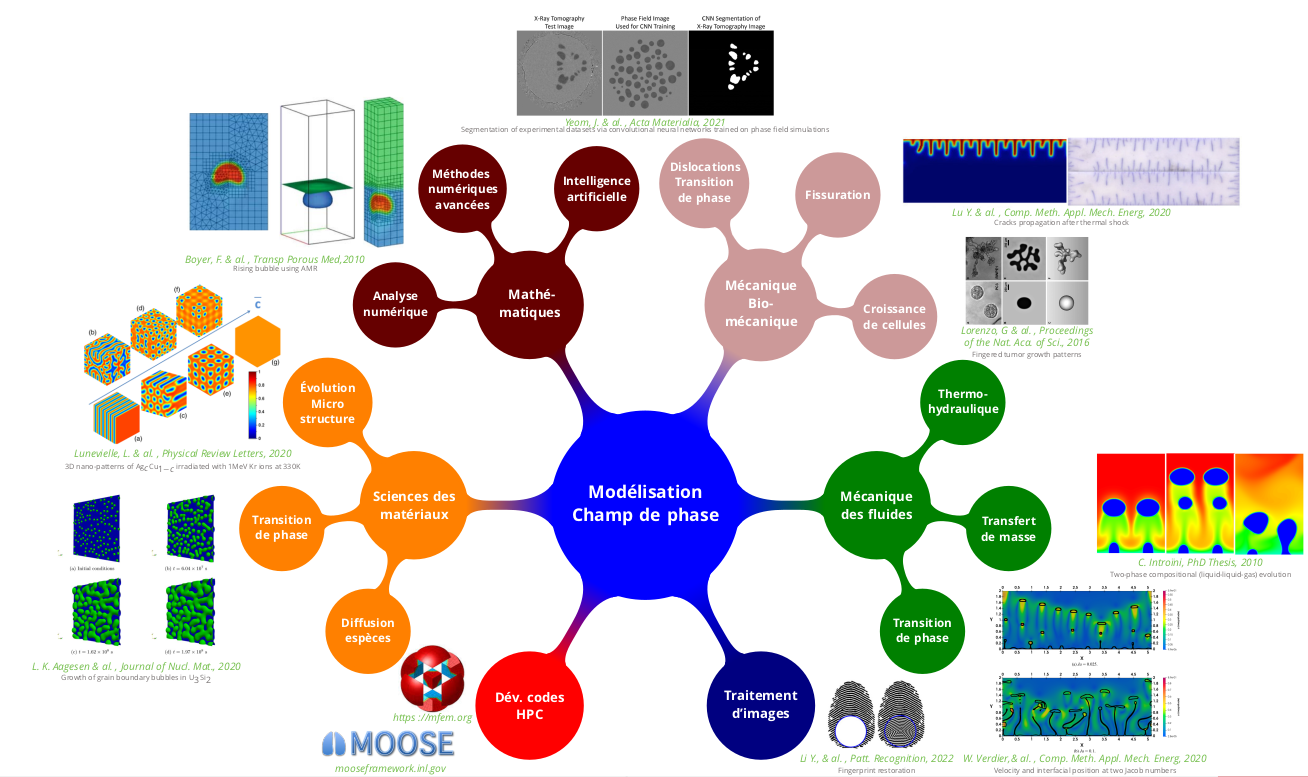
\includegraphics[width=0.9\linewidth]{figure/champ_phase}
	\caption[Domaine d'application de la méthode champ de phase]{Domaine d'application de la méthode champ de phase, tirée de \cite{introini_suivi_nodate}}
	\label{fig:champphase}
\end{figure} 
\section{Equation de Cahn-Hilliard généralisée}
Comme expliqué précédemment la méthode de champ de phase repose sur le suivi d'une variable de phase (ou paramètre d'ordre) noté $\phi_i$ pour la phase $i$ et contraint tel que : 
\begin{equation}
\sum_i \phi_i =1
\end{equation} 
ainsi pour $N$ phase on a :
\begin{equation}
\phi_N =1 - \sum_{i=1}^{N-1} \phi_i
\end{equation} 
Ainsi pour un mélange à $N$ composant on suit uniquement $N-1$ phases.
L'équation de Cahn-Hillard pour $N$ composants, avec $i\in \{1,..,N \}$
\begin{equation}
\cfrac{\partial \phi_i}{\partial t} + \nabla \cdot \mathbf{u}\phi_i=  \nabla \cdot \left(\sum_{j=1}^{N-1} M_{ij} \nabla \frac{\partial \mathcal{F}}{\partial \phi_j} \right)
\end{equation}
avec : $M_{ik}$ la mobilité (paramètre cinétique),  $\phi$ le paramètre d'ordre. \\
on définit le potentiel chimique $\tilde\mu$ tel que : \begin{equation}
\mathcal{F} = \int_{\mathcal{V}}f_0(\bm{\phi},\mathbf{x},t)- \sum_{i=1}^{N-1}\sum_{j=1}^{N-1}\frac{\kappa_{ij}}{2}\nabla \phi_i \cdot \nabla \phi_j dV
\end{equation}
Où le premier terme représente la densité d'énergie liée au volume et le second terme l'énergie liée aux interfaces. $\kappa$ est alors un coefficient de gradient. \\
De tel sorte que : 
\begin{equation}\label{eq_potentiel}
	\frac{\partial \mathcal{F}}{\partial \phi_j} = \frac{\partial f_0}{\partial \phi_j} -\sum_k \kappa_{jk} \Delta \phi_k = \tilde{\mu}_j
\end{equation}
avec $\tilde{\mu}$ le potentiel chimique. \\
Dans le cas où $\doubleoverline{\kappa}$ = $\doubleoverline{0}$ on retrouve une équation d'advection-diffusion classique, dans le cas contraire on obtient une équation d'ordre 4. Une des principale difficulté dans la mise en place de méthode champ de phase repose sur le paramétrage des simulations.
\section{Couplage avec les équations de Navier-Stokes incompressible}
Dans le cadre de cette étude les équations de Cahn-Hilliard sont couplées aux équations de conservation de masse et de quantité de mouvement imcompressible avec l'hypothèse de Boussinesq. On rappel les équations de Navier-Stokes avec ces hypothèses :
\begin{align}
&\nabla \cdot \mathbf{u} = 0\\
&\rho(\bm{\phi}) \left (\frac{\partial \mathbf{u}}{\partial t} + (\mathbf{u} \cdot {\nabla})\mathbf{u}\right) = -{\nabla} P +\eta(\bm{\phi}){\Delta} \mathbf{u}+\sum_{i=1}^{N-1} \tilde\mu_i{\nabla} \phi_i + \rho(\bm{\phi}) \mathbf{g}
\end{align}
avec $\mathbf{u}$ la vitesse, $P$ la pression, $\tilde{\mu_i}$ le potentiel chimique du composant $i$,$\mathbf{g} = -g \mathbf{e_z}$,$\eta$ la viscosité cinématique,$\rho$ la masse volumique\\
La densité est alors calculé : 
\begin{equation}
	\rho(\bm{\phi}) = \rho_0\left(1+\sum_{i=1}^{N-1}\beta_i \phi_i\right)
\end{equation}
Les paramètres $\beta$ sont à déterminer en fonction du système étudié, $\rho_0$ correspond à une masse volumique de référence. L'équation de Cahn-Hilliard étant d'ordre 4, une résolution implicite est préférée pour la suite de ce travail.
\section{Paysage thermodynamique analytique}
L'objectif est de déterminer le paramètre de densité d'énergie liée au volume $f_0$. Dans l'hypothèse de température et pression constante on écrit : 
\begin{equation}
	f_0 = \alpha g^{liq}
\end{equation}
Avec $\alpha$ un pré-facteur correctif et $g^{liq}$ l'énergie libre de Gibbs par unité de volume. On définit également un pseudo grand potentiel correspondant à l'énergie nécessaire pour changer de minimum d'énergie.
\begin{equation}
\Omega^{\star} =\Omega - \Omega^{eq} =  {g}^{liq} - \sum_i \tilde{\mu}_i^{eq}\phi_i - \left( {g}^{liq,eq} -  \sum_i \tilde{\mu}_i^{eq}\phi_i^{eq} \right) 
\end{equation}
Les bases thermodynamiques étant peu développées aux points d'intérêt (Température supérieure à 2000 \textdegree C) on cherche à définir ce potentiel grâce à une formulation analytique que l'on note :
\begin{equation}
	\Omega^{\star}  = P^{dis} \times P^{cont}
\end{equation}
Où $P^{dis}, P^{cont}$ représente deux paraboloïdes correspondant à la phase dispersée et continue. Dans le cas ternaire, avec les éléments $A$ et $B$, les paraboloïdes sont de la forme : 

\begin{multline}
	P^{k}=\left(\frac{\co{\theta^{k}}(\phi_{A}-\phi_{A}^{eq,k}) + \sinus{\theta^{k}}(\phi_{B}-\phi_{B}^{eq,k})}{a_{A}^{k}}\right)^{2}+\\ \left(\frac{-\sinus{\theta^{k}}(\phi_{A}-\phi_{A}^{eq,k}) + \co{\theta^{k}}(\phi_{B}-\phi_{B}^{eq,k})}{a_{B}^{k}}\right)^{2}
	\label{eq:paraboloid_general_}
\end{multline} 
Avec $k = \{disp,cont\}$ la phase (dispersée ou continue), $a_A$ (respectivement $a_B$) le demi-grand (resp petit) puits, $theta_k$ l'angle de rotation associé au puits de la phase $k$\\
On cherche alors à tracer ce paysage. \\
On retrouve dès lors le potentiel chimique grâce à la relation :
\begin{equation}\label{calul_potentiel}
	\tilde{\mu}_i = \left.\frac{\partial g^{liq}}{\partial \phi_i}\right|_{P,T,\phi_{j\neq i}} 
\end{equation}
soit : 
\begin{align*}
	\tilde{\mu}_i &= \frac{\partial}{\partial \phi_i}\left\lbrace 
	\Omega^{\star} + \sum_j \tilde{\mu}_j^{eq}\phi_j + \left( {g}^{liq,eq} -  \sum_j \tilde{\mu}_j^{eq}\phi_j^{eq} \right)\right\rbrace \\
	&= \frac{\partial \Omega^{\star}}{\partial \phi_i} + \frac{\partial g^{liq,eq}}{\partial \phi_i} + \sum_j \frac{\partial \tilde{\mu}_j^{eq}\left(\phi_j - \phi_j^{eq}\right)}{\partial  \phi_i}
\end{align*}
avec 
\begin{align*}
	& \frac{\partial g^{liq,eq}}{\partial \phi_i} = 0 \\
		& \sum_j \frac{\partial \tilde{\mu}_j^{eq}\left(\phi_j - \phi_j^{eq}\right)}{\partial  \phi_i} = \tilde{\mu}_i^{eq} +\tilde{\mu}_{j\neq i}^{eq} \frac{\partial \phi_{j\neq i}}{\partial \phi_i} = \tilde{\mu}_i^{eq}
\end{align*}
car les variables sont indépendantes. Finalement on écrit :
\begin{equation}
\tilde{\mu}_i =	P^{dis}\frac{\partial P^{cont}}{\partial \phi_i} + P^{cont}\frac{\partial P^{dis}}{\partial \phi_i} + \tilde{\mu}_i^{eq}
\end{equation}
L'objectif est alors de déterminer les paramètres des paraboloïdes pour obtenir des résultats consistants.

\section{Élément de stabilité de phase}
Le calcul du paysage nous permet d'avoir des informations sur l'énergie du système pour une certaine composition, cependant on ne connaît aucunement le nombre de phase du système. On cherche alors à déterminer la phase instable ou les deux éléments sont mélangés. Pour cela on calcul la matrice Hessienne définit tel que : 
\begin{equation}
	\Mb{\doubleoverline{H}}_{g^{liq}} = \left.\frac{\partial^2 g^{liq}}{\partial \phi_i \partial \phi_j}\right|_{T,P,\phi_k\neq i,j}
	=\left.\frac{\partial^2 \Omega^{\star}}{\partial \phi_i \partial \phi_j}\right|_{T,P,\phi_k\neq i,j}
\end{equation}
L'égalité des matrices hessienne du pseudo-grand potentiel et de l'énergie libre de Gibbs est ici immédiate. D'après \cite{aursand_spinodal_2017} les zones spinodale, instable et stable sont définit tel que :
\begin{itemize}
	\item zone stable : $\displaystyle eig\left\{\Mb{\doubleoverline{H}}_{g^{liq}} \right\} > 0$, deux phases coexistent \\ 
	\item spinodale : $\displaystyle \min \left( eig \left\{\Mb{\doubleoverline{H}}_{g^{liq}}\right\} \right) > 0$, décomposition spinodale \\
	\item zone instable : $\displaystyle eig\left\{\Mb{\doubleoverline{H}}_{g^{liq}} \right\} < 0$, une phase en présence \\ 
\end{itemize}
Le calcul des valeurs propres en chaque point du paysage pouvant être coûteux on rappel que par théorème le produit des valeurs propres d'une matrice est égale au déterminant de cette matrice. Ainsi si on note $\lambda_i$ les valeurs propres de $\Mb{\doubleoverline{H}}_{g^{liq}}$ on a :
\begin{equation}
	\det{\Mb{\doubleoverline{H}}_{g^{liq}}} = \prod_i \lambda_i
\end{equation}
Pour le cas ternaire le calcul du déterminant est direct :
\begin{equation}
	\text{det}  \Mb{\doubleoverline{H}}   =  \frac{\partial^2 g^{liq}}{\partial \phi_i^2}
	\frac{\partial^2 g^{liq}}{\partial \phi_j^2}-\left(\frac{\partial^2 g^{liq} }{\partial \phi_i \partial \phi_j} \right)^2
\end{equation}

% ======================================== Fin Document ========================================

% ======================================== Début Listes & Co ========================================


\newpage
\printbibliography
\end{document}
